%%%%%%%%%%%%%%%%%%%%%%%%%%%%%%%%%%%%%%%%%%%%%%%%%%%%%%
% A Beamer template for University of Wollongong     %
% Based on THU beamer theme                          %
% Author: Qiuyu Lu                                   %
% Date: July 2024                                    %
% LPPL Licensed.                                     %
%%%%%%%%%%%%%%%%%%%%%%%%%%%%%%%%%%%%%%%%%%%%%%%%%%%%%%
% Customized for Sharif University of Technology     %
%%%%%%%%%%%%%%%%%%%%%%%%%%%%%%%%%%%%%%%%%%%%%%%%%%%%%%


\documentclass[serif, aspectratio=169]{beamer}
%\documentclass[serif]{beamer}  % for 4:3 ratio
\usepackage[T1]{fontenc}
\usepackage{fourier} % see "http://faq.ktug.org/wiki/uploads/MathFonts.pdf" for other options
\usepackage{hyperref}
\usepackage{latexsym,amsmath,xcolor,multicol,booktabs,calligra}
\usepackage{graphicx,pstricks,listings,stackengine}
\usepackage{lipsum}
\usepackage{ragged2e}
\usepackage{colortbl}
\usepackage{times}
\usepackage{fancyhdr,graphicx,amsmath,amssymb,algorithm,algpseudocode,mathtools,needspace}
\usepackage{tikz}
\usetikzlibrary{positioning}
% For writing comments that are aligned to the left side
\makeatletter
\NewDocumentCommand{\LeftComment}{s m}{%
    \Statex \IfBooleanF{#1}{\hspace*{\ALG@thistlm}}\(\triangleright\) #2}
\makeatother
% To manually indent states in algorithmicx
\newcommand{\IndState}{\State\hspace{\algorithmicindent}}
% To make breakable algorithms
\makeatletter
\newenvironment{nofloatalgorithmic}[2][0]
{
    \par
    \needspace{\dimexpr\baselineskip+6.8pt}
    \noindent
    \hrule height.8pt depth0pt \kern2pt
    \refstepcounter{algorithm}
    \addcontentsline{loa}{algorithm}{\numberline{\thealgorithm}#2}
    \noindent\textbf{\fname@algorithm~\thealgorithm} #2\par
    \kern2pt\hrule\kern2pt
    \begin{algorithmic}[#1]
}
{
    \end{algorithmic}
    \nobreak\kern2pt\hrule\relax
}
\makeatother
% To make vertical arrow
\newcommand\vertarrowbox[3][6ex]{%
    \begin{array}[t]{@{}c@{}} #2 \\
    \left\uparrow\vcenter{\hrule height #1}\right.\kern-\nulldelimiterspace\\
    \makebox[0pt]{\scriptsize#3}
    \end{array}%
}
\DeclareMathOperator*{\argmax}{argmax}

\author{Ali Sharifi-Zarchi}
\title{Machine Learning (CE 40717)}
\subtitle{Fall 2025}
\institute{
    CE Department \\
    Sharif University of Technology
}
%\date{\small \today}
% \usepackage{UoWstyle}
\usepackage{SUTstyle}

% defs
\def\cmd#1{\texttt{\color{red}\footnotesize $\backslash$#1}}
\def\env#1{\texttt{\color{blue}\footnotesize #1}}
\definecolor{deepblue}{rgb}{0,0,0.5}
\definecolor{deepred}{RGB}{153,0,0}
\definecolor{deepgreen}{rgb}{0,0.5,0}
\definecolor{halfgray}{gray}{0.55}

\lstset{
    basicstyle=\ttfamily\small,
    keywordstyle=\bfseries\color{deepblue},
    emphstyle=\ttfamily\color{deepred},    % Custom highlighting style
    stringstyle=\color{deepgreen},
    numbers=left,
    numberstyle=\small\color{halfgray},
    rulesepcolor=\color{red!20!green!20!blue!20},
    frame=shadowbox,
}


\begin{document}

    \begin{frame}
        \titlepage
        \vspace*{-0.6cm}
        \begin{figure}[htpb]
            \begin{center}
                
\includegraphics[keepaspectratio, scale=0.25]{pic/sharif-main-logo.png}
            \end{center}
        \end{figure}
    \end{frame}

    \begin{frame}
        \tableofcontents[sectionstyle=show,
            subsectionstyle=show/shaded/hide,
            subsubsectionstyle=show/shaded/hide]
    \end{frame}


%------------------------------------------------
    \begin{frame}{How Machines Learn to Decide}
        \begin{itemize}\itemsep1.2em
        \item Classification is a \textbf{decision-making process}.
        A model learns from past examples how to assign new inputs to categories.

        \item Examples from daily life:
        \begin{itemize}
            \item A doctor examines an X-ray and determines if it shows pneumonia.
            \item A bank reviews a transaction and flags it as legitimate or fraudulent.
            \item Your phone sorts messages into \textit{Primary}, \textit{Promotions}, or \textit{Spam}.
        \end{itemize}

        \item In all cases:
        \begin{itemize}
            \item The input is described by measurable features.
            \item The output is a predicted class.
            \item The model learns patterns or rules to separate classes.
        \end{itemize}

        \item Key idea: Classification is about learning general patterns, not memorizing examples.
        \end{itemize}
    \end{frame}

%------------------------------------------------
    \begin{frame}{How Classification Works}
        \begin{itemize}\itemsep1em
        \item We start with a training dataset:
        \[
            D = \{(\mathbf{x}^{(i)}, y^{(i)})\}_{i=1}^{N}
        \]
        where $\mathbf{x}^{(i)}$ is a feature vector and $y^{(i)}$ is the class label.
        \item The model learns a function that maps features to classes:
        \[
            f: \mathbb{R}^n \rightarrow \{1, 2, \dots, K\}
        \]
        \item During training, the algorithm identifies patterns that separate one class from another.
        \item After training, the model can predict the class of new, unseen inputs.
        \end{itemize}
    \end{frame}

%------------------------------------------------
    \begin{frame}{Case Study: Predicting Diabetes (Concept)}
        \begin{itemize}\itemsep1em
        \item Goal: Predict whether a patient has diabetes based on medical measurements.
        \item Dataset: Pima Indians Diabetes Dataset.
        \item Input features: Glucose level, blood pressure, BMI, age, etc.
        \item Output label:
        \[
            y =
            \begin{cases}
                1, & \text{Diabetic (Positive)}\\
                0, & \text{Non-diabetic (Negative)}
            \end{cases}
        \]
        \item Importance: Early prediction supports prevention and treatment.
        \end{itemize}
    \end{frame}

%------------------------------------------------
    \begin{frame}{Case Study: Diabetes Dataset Table}
        \begin{table}[]
            \resizebox{\textwidth}{!}{%
                \begin{tabular}{|c|c|c|c|c|c|c|c|c|c|}
                    \hline
                    \rowcolor[HTML]{C0C0C0}
                    \cellcolor[HTML]{000000}\textcolor{white}{\#} & Pregnancies & Glucose & Blood Pressure & Skin Thickness & Insulin & Pedigree & Age & BMI & Label \\ \hline
                    1 & 6 & 148 & 72 & 35 & 0 & 0.627 & 50 & 33.6 & \cellcolor[HTML]{FE0000}\textcolor{white}{Positive} \\ \hline
                    2 & 1 & 85 & 66 & 29 & 0 & 0.351 & 31 & 26.6 & \cellcolor[HTML]{32CB00}\textcolor{white}{Negative} \\ \hline
                    3 & 0 & 137 & 40 & 35 & 168 & 2.288 & 33 & 43.1 & \cellcolor[HTML]{FE0000}\textcolor{white}{Positive} \\ \hline
                    4 & 1 & 89 & 66 & 23 & 94 & 0.167 & 21 & 28.1 & \cellcolor[HTML]{32CB00}\textcolor{white}{Negative} \\ \hline
                    \begin{tabular}[c]{@{}c@{}}.\\ .\\ .\end{tabular} &
                    \begin{tabular}[c]{@{}c@{}}.\\ .\\ .\end{tabular} &
                    \begin{tabular}[c]{@{}c@{}}.\\ .\\ .\end{tabular} &
                    \begin{tabular}[c]{@{}c@{}}.\\ .\\ .\end{tabular} &
                    \begin{tabular}[c]{@{}c@{}}.\\ .\\ .\end{tabular} &
                    \begin{tabular}[c]{@{}c@{}}.\\ .\\ .\end{tabular} &
                    \begin{tabular}[c]{@{}c@{}}.\\ .\\ .\end{tabular} &
                    \begin{tabular}[c]{@{}c@{}}.\\ .\\ .\end{tabular} &
                    \begin{tabular}[c]{@{}c@{}}.\\ .\\ .\end{tabular} &
                    \begin{tabular}[c]{@{}c@{}}.\\ .\\ .\end{tabular} \\ \hline
                \end{tabular}
            }
        \end{table}
    \end{frame}

    \begin{frame}{Classification vs. Regression: Comparison Table}

        \begin{itemize}
            \item Both are \textit{supervised learning} tasks — learn a mapping from inputs to outputs.
            \item \textbf{Regression:} models a \textit{continuous relationship} — how inputs influence a numeric outcome.
            \item \textbf{Classification:} models \textit{decision boundaries or class probabilities} — how inputs determine category membership.

        \end{itemize}

        \begin{center}
            \renewcommand{\arraystretch}{1.5}
            \setlength{\tabcolsep}{4pt}
            \begin{tabular}{|
                    >{\columncolor[HTML]{C0C0C0}}p{2.5cm} |p{4cm}|p{5.5cm}|}
                \hline
                \textbf{Aspect} & \textbf{Regression} & \textbf{Classification} \\ \hline
                \textbf{Output Type} & Continuous value ($\mathbb{R}$) & Discrete class label \\ \hline
                \textbf{Examples} & House price, temperature & Spam detection, sentiment analysis \\ \hline
                \textbf{Evaluation Metrics} & MSE, MAE & Accuracy, Precision, Recall \\ \hline
            \end{tabular}
        \end{center}

    \end{frame}



    \section{Discriminant Functions}



    \begin{frame}{Discriminant Functions in Machine Learning}
        \begin{itemize}\itemsep1.2em
        \item \textbf{Conceptual Overview:}\\
        A discriminant function constitutes a mapping from the feature space to a real-valued score that quantifies the likelihood or confidence of a sample belonging to a specific class.
        \item \textbf{Formal Definition:}\\
        Let $\mathbf{x} \in \mathbb{R}^d$ denote a feature vector. A discriminant function is a function $g(\mathbf{x}) : \mathbb{R}^d \rightarrow \mathbb{R}$ such that larger values of $g(\mathbf{x})$ correspond to stronger evidence for a particular class.
        \item \textbf{Objective:}\\
        Design $g(\mathbf{x})$ to maximize correct classification over a given dataset.
        \end{itemize}
    \end{frame}




    \begin{frame}{Classification Using Discriminant Functions}
        \begin{itemize}\itemsep1.5em
        \item \textbf{Binary Classification:}\\
        \begin{itemize}
            \item Consider two discriminant functions $g_1(\mathbf{x})$ and $g_2(\mathbf{x})$ corresponding to classes $C_1$ and $C_2$, respectively.
            \item The predicted class $\hat{y}$ is determined by the criterion:
            \[
                \hat{y} =
                \begin{cases}
                    C_1 & \text{if } g_1(\mathbf{x}) > g_2(\mathbf{x}) \\
                    C_2 & \text{otherwise.}
                \end{cases}
            \]
        \end{itemize}

        \item \textbf{Multi-Class Classification:}\\
        \begin{itemize}
            \item For $k$ classes, compute $g_i(\mathbf{x})$ for each class $C_i$, $i=1,\dots,k$.
            \item Assign $\mathbf{x}$ to the class corresponding to the maximal discriminant value:
            \[
                \hat{y} = \arg \max_{i} g_i(\mathbf{x})
            \]
        \end{itemize}

        \item \textbf{Interpretation:}
        The discriminant function serves as a quantitative measure of class membership confidence.
        \end{itemize}
    \end{frame}


    \begin{frame}{Decision Boundary}
        \begin{itemize}
            \item \justifying \textbf{Definition}: A dividing hyperplane that separates different classes in a feature space, also known as "Decision Surface".
            \medskip
            \begin{figure}
                \centering
                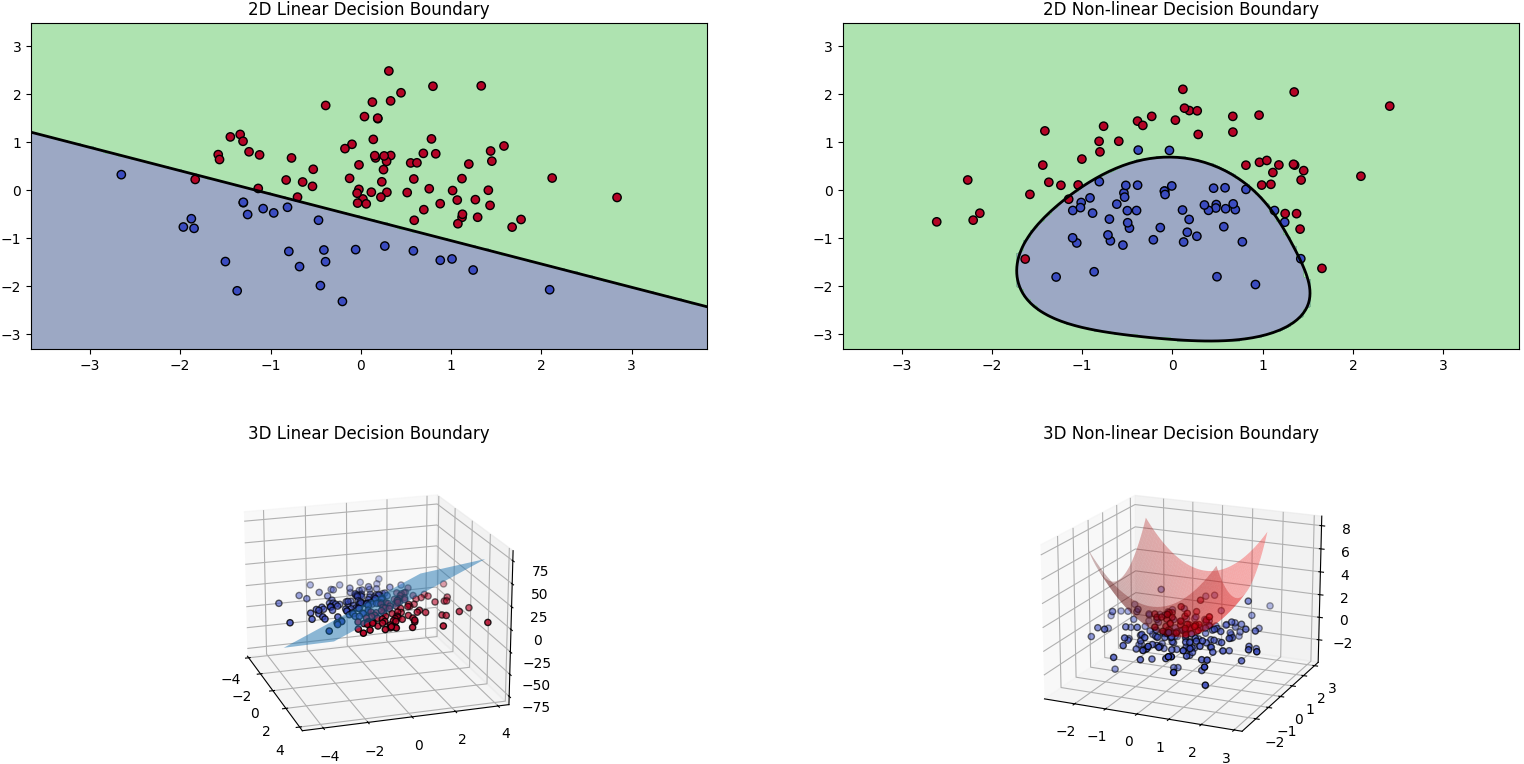
\includegraphics[width=.85\linewidth]{pic/Figure_24.png}
            \end{figure}
        \end{itemize}
    \end{frame}




    \section{Linear Classifiers}

    \begin{frame}{Linear Classifiers}
        \begin{itemize}\itemsep1.5em
        \item \justifying \textbf{Definition:}\\
        Linear classifiers assign class labels using a decision function that is linear in the feature vector $\mathbf{x} \in \mathbb{R}^d$, or linear in a set of transformed features of $\mathbf{x}$.
        \item \justifying \textbf{Linearly separable data:}\\
        Data points that can be perfectly separated by a linear decision boundary.
        \item \textbf{General form:}
        \[
            g(\mathbf{x}) = \mathbf{w}^T \mathbf{x} + w_0,
        \]
        where $\mathbf{w}$ defines the orientation of the decision surface and $w_0$ determines its position.
        \end{itemize}
    \end{frame}


    \begin{frame}{Two-Category Classification}
        \minipage{.5\textwidth}
        \begin{itemize}\itemsep1.2em
        \item \textbf{Linear discriminant:}
        \[
            g(\mathbf{x}) = \mathbf{w}^T\mathbf{x} + w_0
        \]
        \item \(\mathbf{x} = [x_1, \dots, x_d]^T,\; \mathbf{w} = [w_1, \dots, w_d]^T,\; w_0:\text{ bias}\)
        \item \textbf{Decision rule:}
        \[
            \hat{y} =
            \begin{cases}
                C_1, & \text{if } g(\mathbf{x}) \ge 0 \\
                C_2, & \text{otherwise}
            \end{cases}
        \]
        \item \textbf{Decision surface:} $\mathbf{w}^T\mathbf{x} + w_0 = 0$
        \end{itemize}
        \endminipage
        \hfill
        \minipage{.48\textwidth}
        \begin{figure}[bh]
            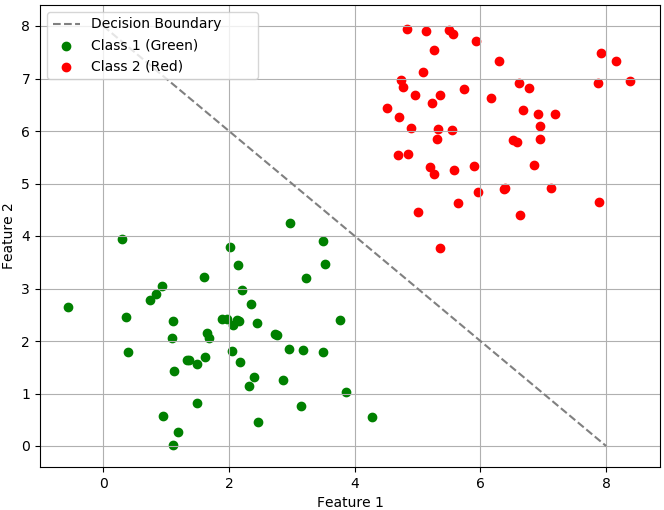
\includegraphics[width=\linewidth]{pic/Figure_1.png}
        \end{figure}
        \endminipage
    \end{frame}


    \begin{frame}{Geometric Properties of Linear Decision Boundaries}
        \begin{itemize}\itemsep1.2em
        \item The decision boundary is a $(d-1)$-dimensional hyperplane in $\mathbb{R}^d$.
        \item \textbf{Properties:}
        \begin{itemize}
            \item Orientation is determined by the normal vector $\mathbf{w}/\|\mathbf{w}\|$.
            \item Bias $w_0$ controls the displacement along the normal vector.
        \end{itemize}
        \item Points on opposite sides of the hyperplane are assigned to different classes.
        \end{itemize}
        \begin{figure}
            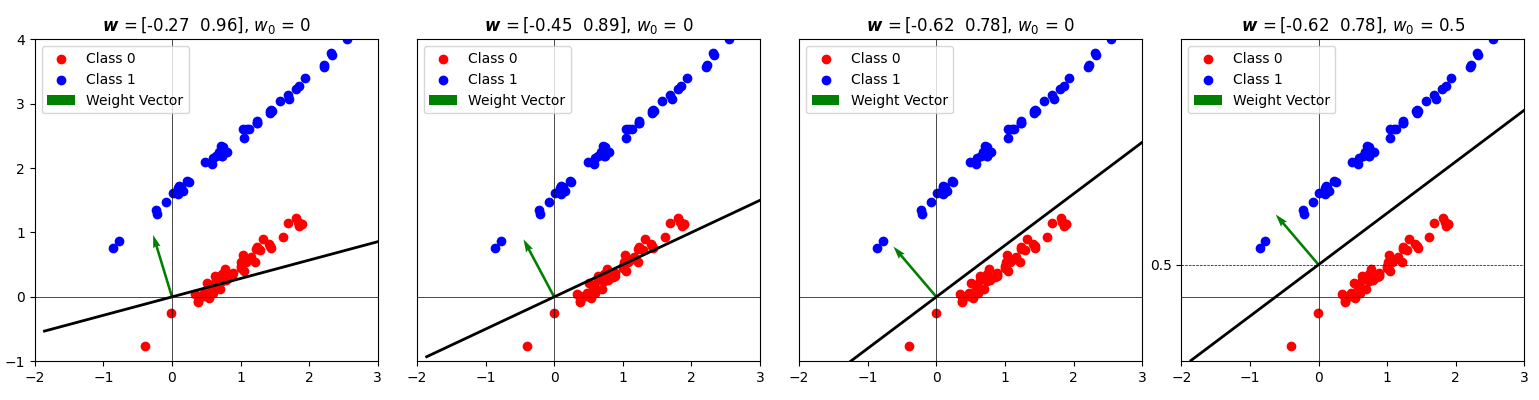
\includegraphics[width=\linewidth]{pic/Figure_25.png}
        \end{figure}
    \end{frame}

    \begin{frame}{Nonlinear Decision Boundaries}
        \minipage{.46\textwidth}
        \begin{itemize}\itemsep1em
        \item \textbf{Problem:}\\ Many datasets cannot be separated by a linear hyperplane.
        \item \textbf{Feature Transformation:}\\ Map input vector $\mathbf{x}$ to a higher-dimensional space $\phi(\mathbf{x})$.
        \item \textbf{Resulting Decision Boundary:}\\ Linear in the transformed space, but nonlinear in the original feature space.
        \end{itemize}
        \endminipage
        \hfill
        \minipage{.5\textwidth}
        \begin{figure}
            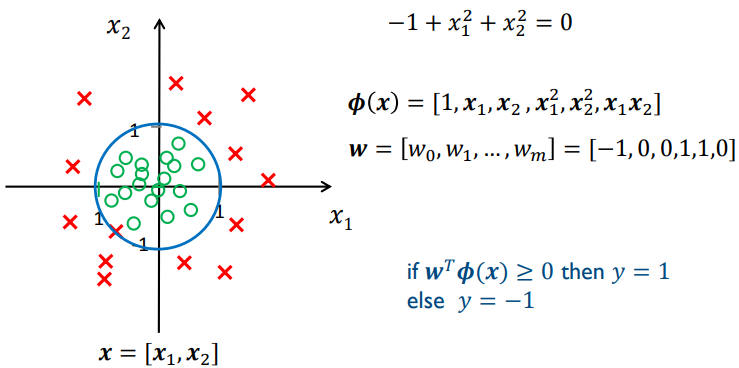
\includegraphics[width=\textwidth]{pic/Figure_10.png}
        \end{figure}
        \endminipage
        \vfill
        \begin{tikzpicture}[remember picture,overlay]
            \node[anchor=south west, xshift=0.1cm, yshift=0.22cm] at (current page.south west) {
                \scriptsize Figure adapted from M. Soleymani, Machine Learning course, Sharif University of Technology.
            };
        \end{tikzpicture}
    \end{frame}

    \section{Perceptron}

    \begin{frame}{From Biology to Computation}
        \minipage{.6\textwidth}
        \begin{itemize}
            \item \textbf{Biological Inspiration:}
            \medskip
            \begin{itemize}\itemsep1em
            \item \justifying The human brain consists of interconnected cells called \textbf{neurons}, each transmitting signals to others through electrical impulses.
            \item \justifying Each neuron receives inputs, processes them, and produces an output signal.
            \item \justifying This biological structure inspired the design of artificial computational models known as \textbf{perceptrons}.
            \end{itemize}
        \end{itemize}
        \endminipage
        \hfill
        \minipage{.38\textwidth}
        \centering
        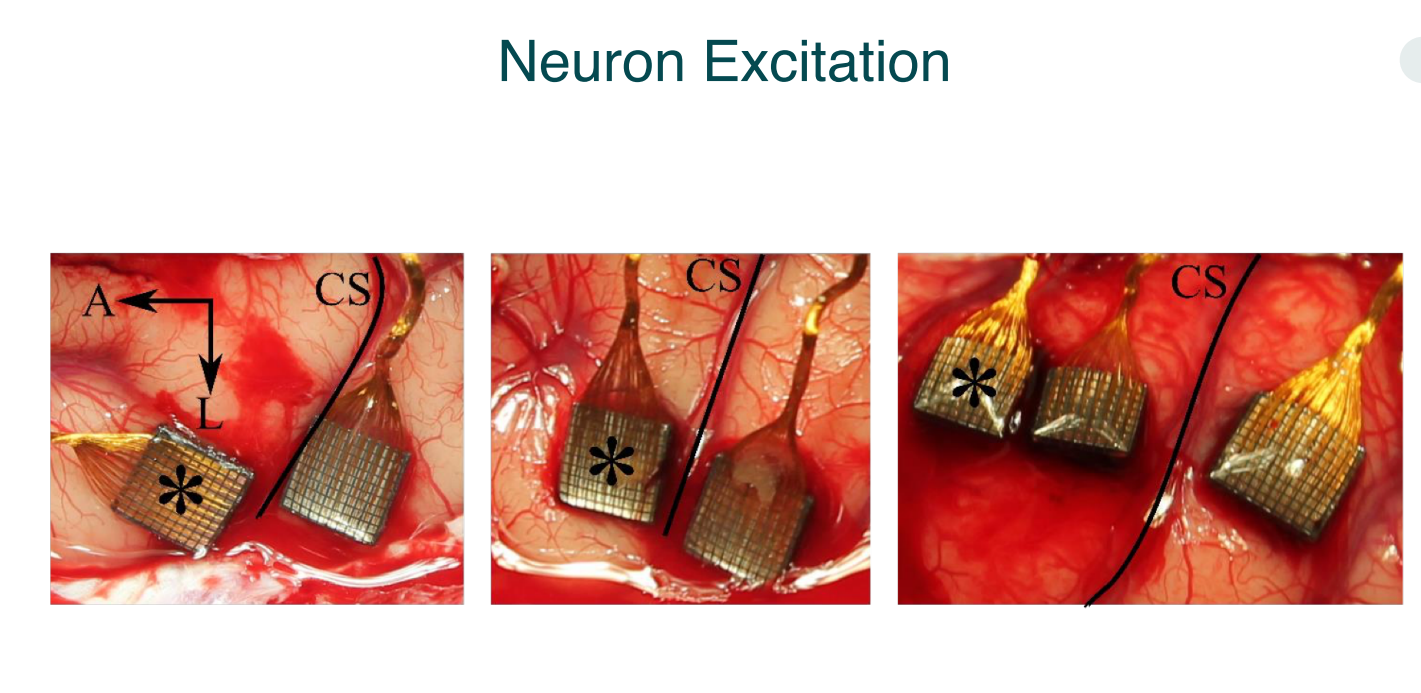
\includegraphics[width=\linewidth]{pic/Figure_38.png}
        \vspace{0.3em}
        \scriptsize Figure adapted from Nason et al., Nature Biomedical Engineering, 2020.
        \endminipage
    \end{frame}



%---------------------------------------------
    \begin{frame}{From Neuron to Perceptron}
        \minipage{.58\textwidth} \begin{itemize} \item \textbf{Abstracting a Neuron:} \medskip \begin{itemize}\itemsep1em \item Biological neurons combine multiple inputs, each with a strength (synapse). \item Similarly, a perceptron multiplies each input by a \textbf{weight}, sums them, adds a \textbf{bias}, and applies an \textbf{activation function}. \item The activation function determines whether the perceptron “fires” (outputs \(1\)) or stays “inactive” (outputs \(0\)). \end{itemize} \end{itemize} \endminipage
        \hfill
        \minipage{.42\textwidth}
        \centering
        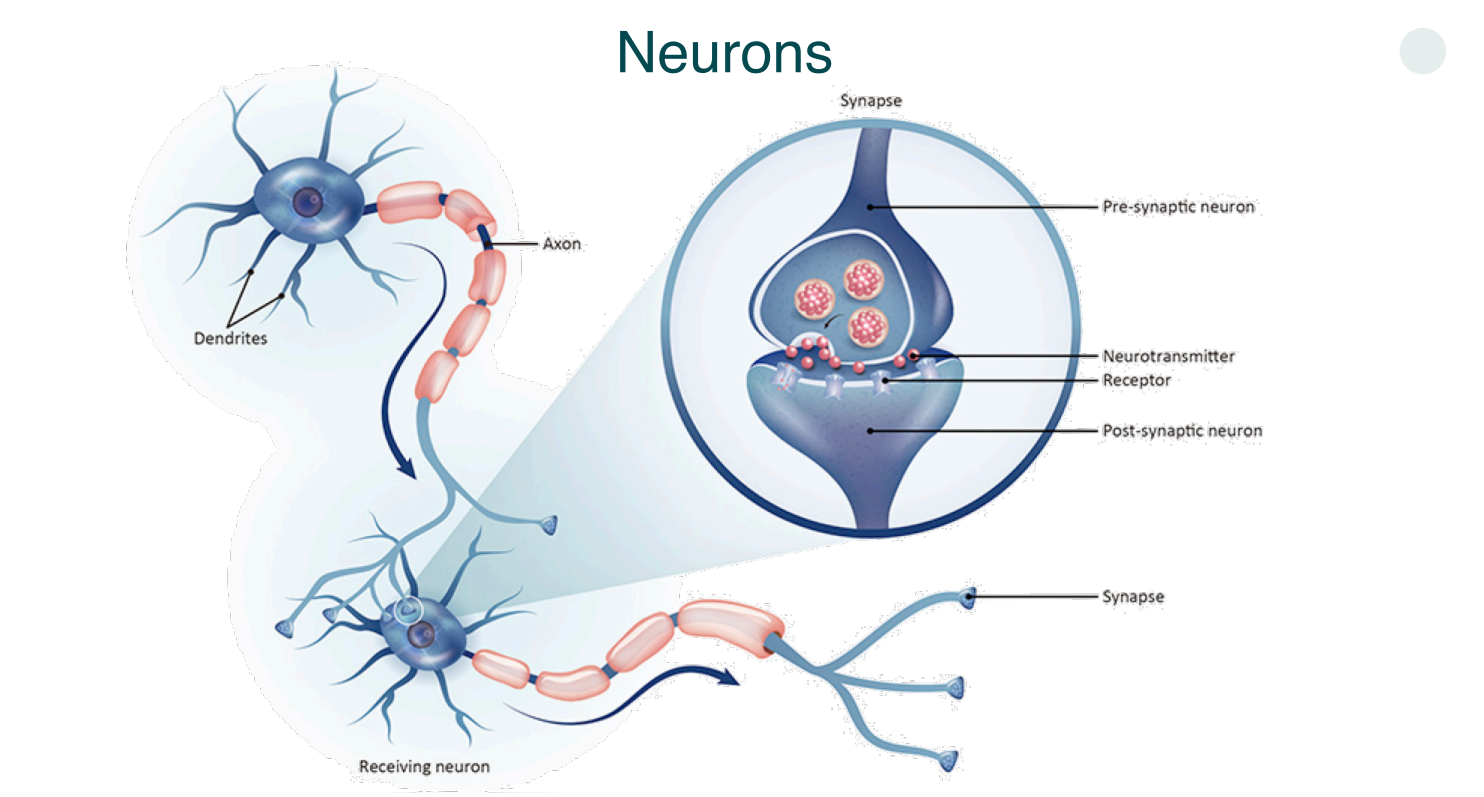
\includegraphics[width=\linewidth]{pic/Figure_41.png}\\
        \vspace{0.3em}
        \scriptsize Figure adapted from www.genetex.com
        \endminipage

    \end{frame}


%---------------------------------------------
    \begin{frame}{Components of a Perceptron}
        \begin{itemize}\itemsep1em
        \item \textbf{Inputs (\(x_1, x_2, \dots, x_n\))} – the feature values.
        \item \textbf{Weights (\(w_1, w_2, \dots, w_n\))} – importance of each feature.
        \item \textbf{Bias (\(b\))} – adjusts the threshold for activation.
        \item \textbf{Weighted Sum:}
        \[
            z = \sum_{i=1}^n w_i x_i + b = \mathbf{w}^T \mathbf{x} + b
        \]
        \item \textbf{Activation Function (\(f\))} – transforms \(z\) into output:
        \[
            y = f(z)
        \]
        \end{itemize}
    \end{frame}

%---------------------------------------------
    \begin{frame}{Activation Functions — Step & Sigmoid}
        \begin{itemize}\itemsep0.8em
        \item \textbf{Step Function:}
        \[
            f(z) =
            \begin{cases}
                1 & z \ge 0 \\
                0 & z < 0
            \end{cases}
        \]
        Classic perceptron; non-differentiable.

        \item \textbf{Sigmoid Function:}
        \[
            f(z) = \frac{1}{1 + e^{-z}}
        \]
        Smooth output (0–1); differentiable; may saturate for large \(|z|\).
        \end{itemize}
    \end{frame}

%---------------------------------------------
    \begin{frame}{Activation Functions — ReLU & Variants}
        \begin{itemize}\itemsep0.8em
        \item \textbf{ReLU:}
        \[
            f(z) = \max(0, z)
        \]
        Passes positives, zeros negatives; fast & stable training.

        \item \textbf{Leaky ReLU:}
        \[
            f(z) = \max(0.01z, z)
        \]
        Allows small gradient for negative inputs.

        \item \textbf{Tanh:}
        \[
            f(z) = \tanh(z)
        \]
        Output in \([-1, 1]\); smooth and zero-centered.
        \end{itemize}
    \end{frame}


%---------------------------------------------
    \begin{frame}{Activation Functions}
        \begin{figure}
            \centering
            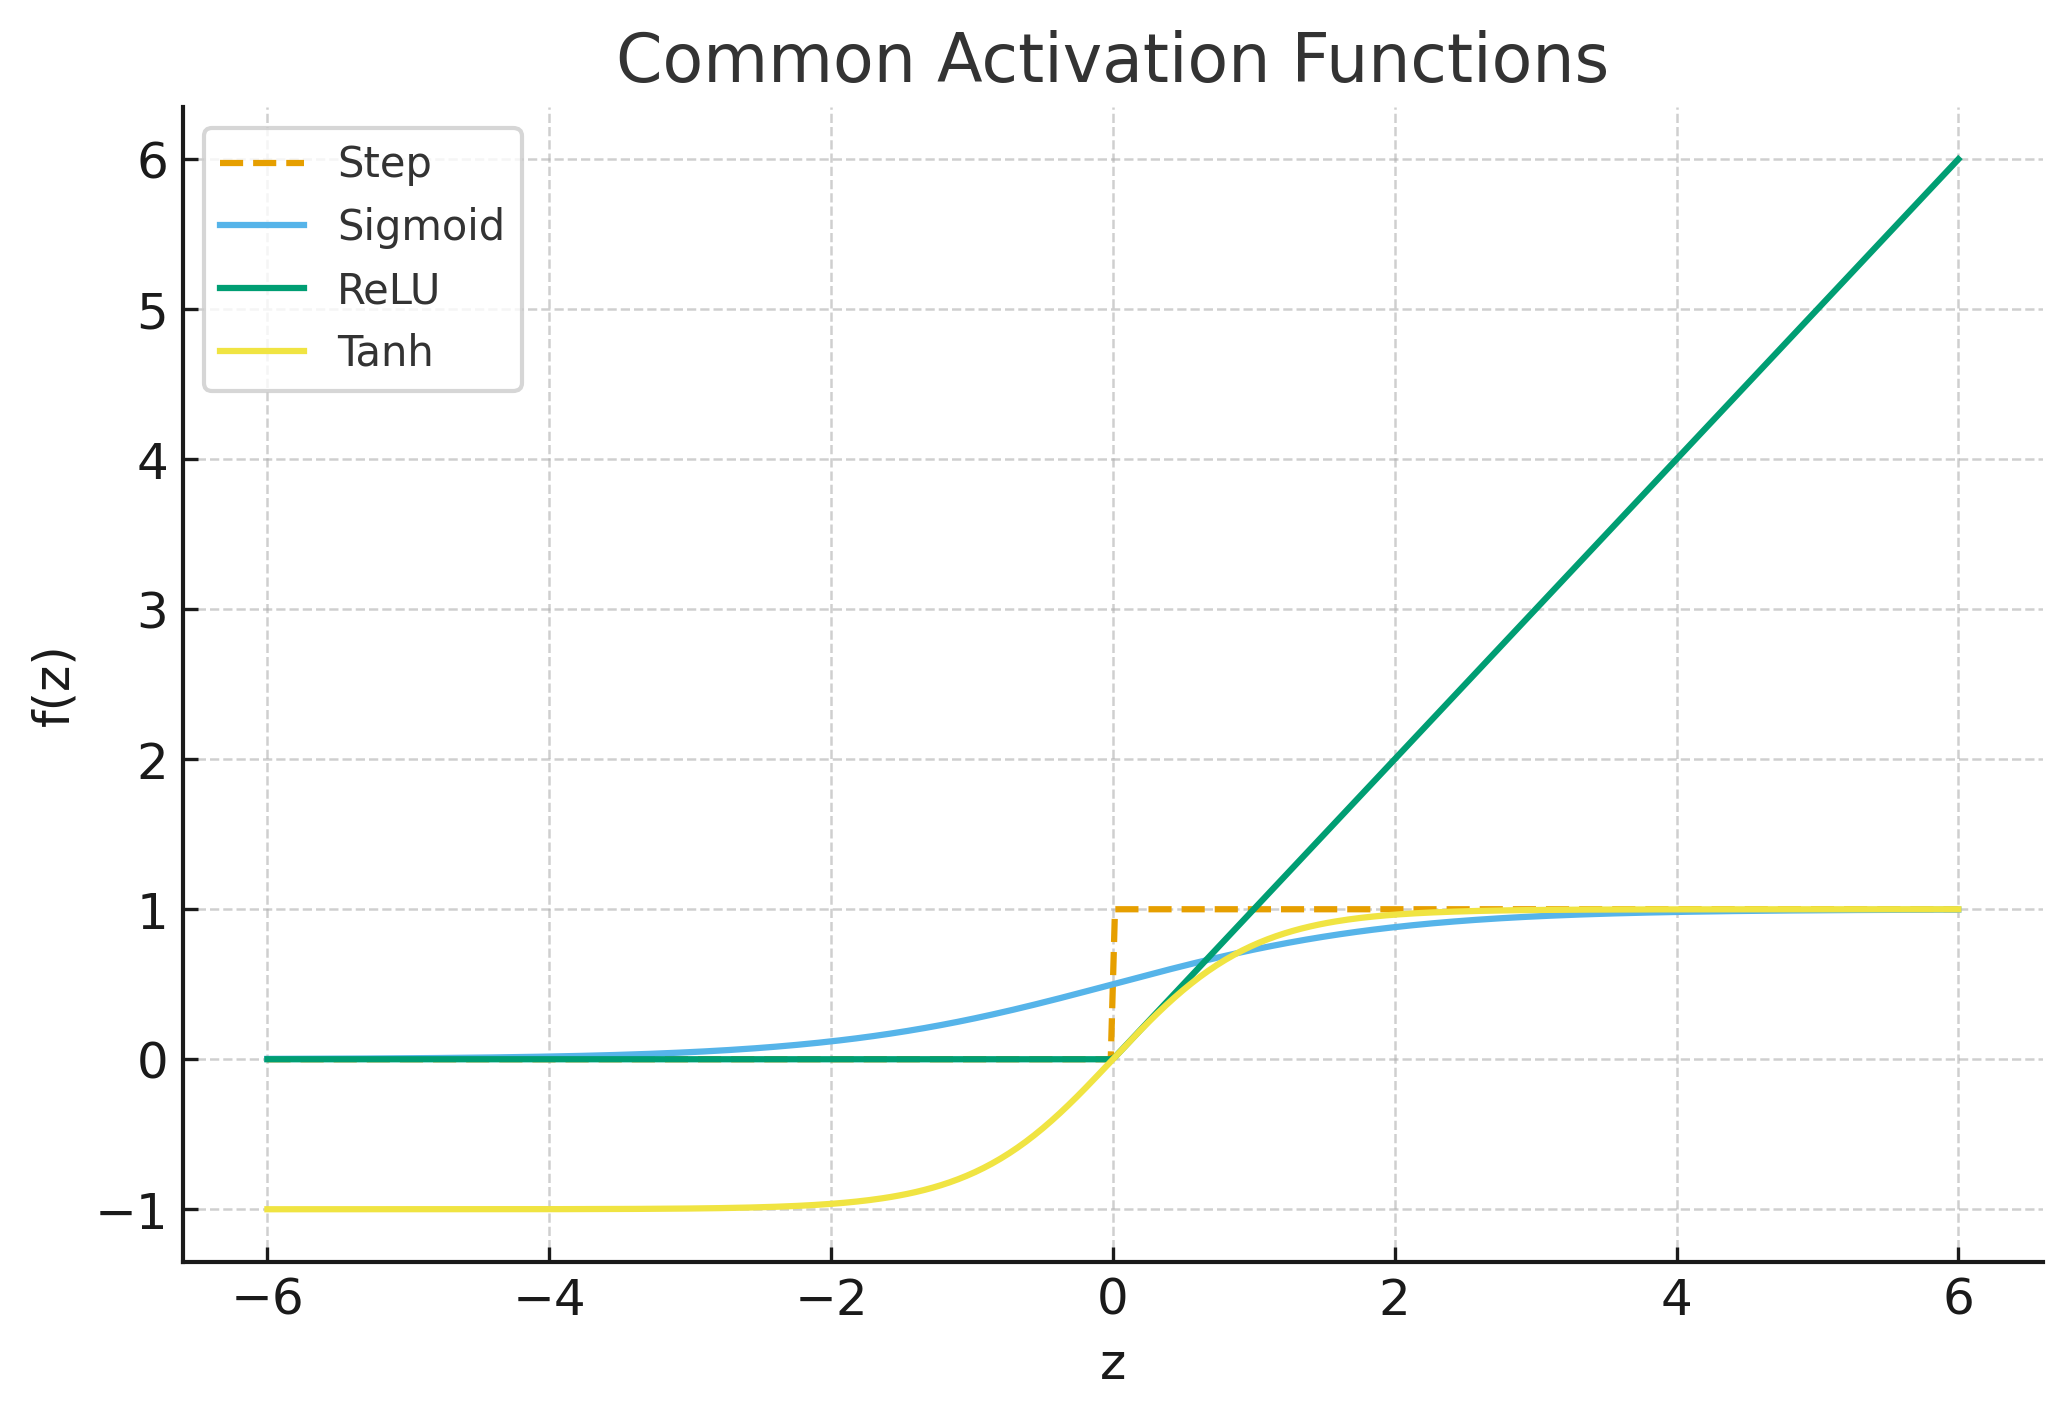
\includegraphics[width=0.7\linewidth]{pic/Figure_40.png}
        \end{figure}
    \end{frame}

%---------------------------------------------
    \begin{frame}{Mathematical Model of a Perceptron}
        \minipage{.58\textwidth}
        \begin{itemize}\itemsep1em
        \item \textbf{Computation Rule:}
        \[
            y = f(\mathbf{w}^T \mathbf{x} + b)
        \]
        \item \textbf{Explanation:}
        \begin{itemize}
            \item \( \mathbf{x} \): input vector of features.
            \item \( \mathbf{w} \): weight vector determining importance.
            \item \( b \): bias, controlling threshold.
            \item \( f \): activation function.
        \end{itemize}
        \item The perceptron outputs \(1\) if the weighted sum exceeds the threshold, otherwise \(0\).
        \end{itemize}
        \endminipage
        \hfill
        \minipage{.38\textwidth}
        \centering
        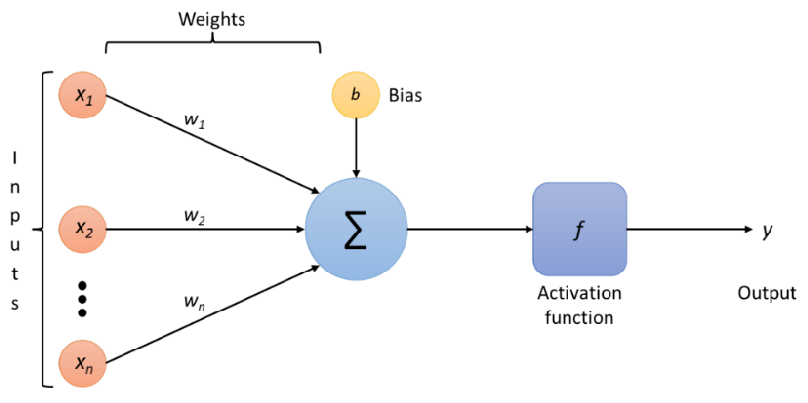
\includegraphics[width=\linewidth]{pic/Figure_39.png}\\
        \vspace{0.3em}
        \scriptsize Figure Adapted from Sánchez et al. (2022)
        \endminipage
    \end{frame}

%---------------------------------------------
    \begin{frame}{Linear Decision Boundary}
        \minipage{.66\textwidth}
        \begin{itemize}\itemsep1em
        \item The perceptron defines a \textbf{linear boundary}:
        \[
            \mathbf{w}^T \mathbf{x} + b = 0
        \]
        \item All points on one side of this line (or hyperplane) belong to class \(C_1\); others to class \(C_2\).
        \item Example of linearly separable problems:
        \begin{itemize}
            \item Logical AND
            \item Logical OR
        \end{itemize}
        \end{itemize}
        \endminipage
        \hfill
        \minipage{.3\textwidth}
        \centering
        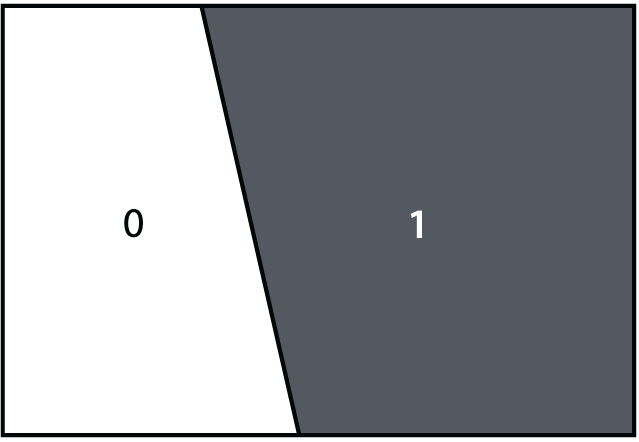
\includegraphics[width=\linewidth]{pic/Figure_20.png}
        \scriptsize Example: linear separation in 2D space.
        \endminipage
    \end{frame}

%---------------------------------------------
    \begin{frame}{Limitation of a Single Perceptron}
        \minipage{.6\textwidth}
        \begin{itemize}\itemsep1em
        \item A single perceptron can only solve \textbf{linearly separable} problems.
        \item It fails on tasks like the \textbf{XOR problem}, where no straight line can divide the two classes.
        \item To handle more complex patterns, we need to move beyond simple linear models.
        \end{itemize}
        \endminipage
        \hfill
        \minipage{.36\textwidth}
        \centering
        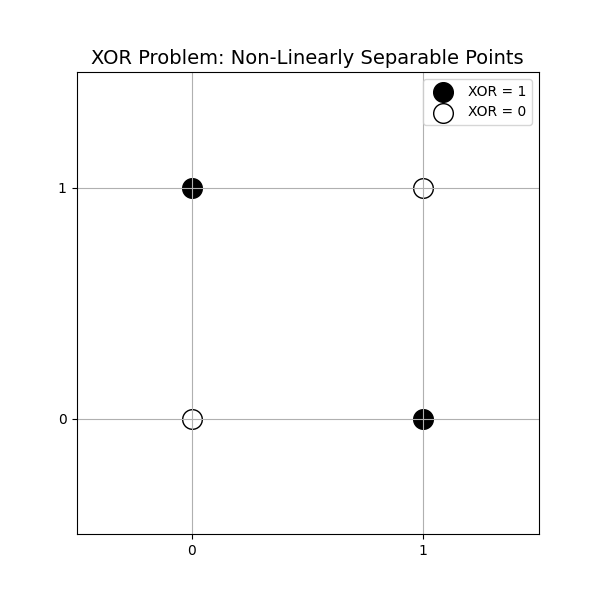
\includegraphics[width=\linewidth]{pic/Figure_23.png}
        \scriptsize XOR problem — not linearly separable.
        \endminipage
    \end{frame}

%---------------------------------------------
    \begin{frame}{Feature Engineering: Manually Creating New Views of Data}
        \begin{itemize}\itemsep1em
        \item \textbf{Feature engineering} means designing or transforming input variables
        so that a model can better capture patterns in the data.
        \item When data isn’t linearly separable, we can transform it into a higher-dimensional space.
        \item Example:
        \[
            (x_1, x_2) \rightarrow (x_1, x_2, x_1x_2)
        \]
        \item The new feature \(x_1x_2\) helps separate XOR data using a simple linear classifier.
        \item In essence, we make the data easier for the model to understand.
        \end{itemize}
    \end{frame}
%---------------------------------------------
    \begin{frame}{Multi-Layer Perceptrons}
        \minipage{.6\textwidth}
        \begin{itemize}\itemsep1em
        \item \textbf{Automatic feature learning:} MLPs extract useful representations from data without manual engineering.
        \item Layers are stacked to capture \textbf{nonlinear relationships}:
        \[
            \text{Input Layer} \rightarrow \text{Hidden Layer(s)} \rightarrow \text{Output Layer}
        \]
        \item Hidden layers use \textbf{nonlinear activations} (e.g., ReLU, Sigmoid) to form flexible decision boundaries.
        \item Each layer builds on the previous, progressively learning more abstract features.
        \end{itemize}
        \endminipage
        \hfill
        \minipage{.38\textwidth}
        \centering
        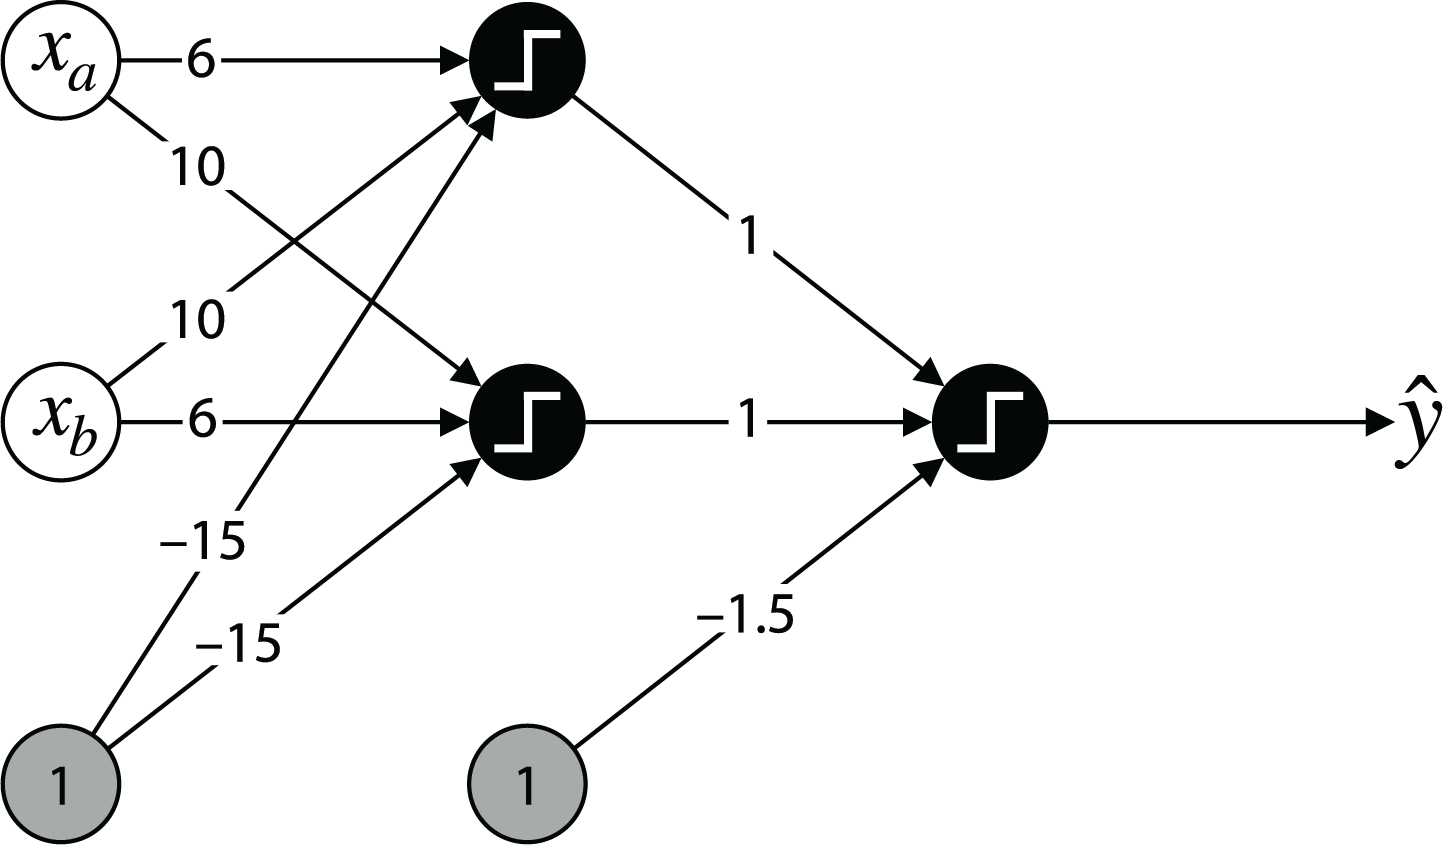
\includegraphics[width=\linewidth]{pic/Figure_21.png}
        \vspace{0.3em}
        \scriptsize Figure adapted from mriquestions.com.
        \endminipage
    \end{frame}

%---------------------------------------------
    \begin{frame}{Key Takeaways}
        \begin{itemize}\itemsep1em
        \item Perceptrons perform linear classification — simple but limited.
        \item \textbf{Feature engineering} helps models handle nonlinear patterns by transforming inputs.
        \item Manual feature design is powerful but often impractical for high-dimensional data.
        \item \textbf{Multi-Layer Perceptrons} learn these transformations automatically through hidden layers and nonlinear activations.
        \item Deep networks are, in many ways, models that learn to do their own feature engineering.
        \end{itemize}
    \end{frame}


    \section{Cost Functions}


    \begin{frame}{Cost Functions}
        \begin{itemize}
            \item \textbf{Understanding the Goal}
            \medskip
            \begin{itemize}\itemsep1em
            \item In the perceptron, we use \( \mathbf{w}^T \mathbf{x} \) to make predictions.
            \item Goal is to find the optimal \(\mathbf{w}\) so that the predicted labels match the true labels as much as possible.
            \item To achieve this, we define a cost function, which measures the \textbf{difference} between \textbf{predicted} and \textbf{actual} labels.
            \item Finding discriminant functions (\(\mathbf{w}^T\), \(w_0\)) is framed as minimizing a cost function.
            \smallskip
            \begin{itemize}\itemsep0.8em
            \item Based on training set \(D \, = \, \{(\mathbf{x}^{(i)},\, y^{(i)})\}^N_{i=1},\) a cost function \(J(\mathbf{w})\) is defined.
            \item Problem converts to finding optimal \(\hat{g}(\mathbf{x}) \, = \, g(\mathbf{x; \hat{w}})\) where \[\mathbf{\hat{w}} \, = \, \arg \min_{\mathbf{w}}J(\mathbf{w})\]
            \end{itemize}
            \end{itemize}
        \end{itemize}
    \end{frame}



    \begin{frame}{Sum of Squared Error Cost Function}
        \begin{itemize}
            \item \textbf{Sum of Squared Error (SSE) Cost Function}\itemsep1em
            \medskip
            \begin{itemize}\itemsep0.8em
            \item \textbf{Formula}:
            \(
            J(\mathbf{w}) = \sum_{i=1}^{n} (y^{(i)} - \hat{y}^{(i)})^2 \, , \quad \hat{y}^{(i)} \, = \, \mathbf{w}^T\mathbf{x}^{(i)} \, + \, w_0
            \)
            \item \justifying SSE minimizes the magnitude of the error, which is ideal for regression but \textcolor{red}{irrelevant} for classification.
            \item \justifying If the model predicts close to the true class but not exactly 0 or 1, SSE still shows positive error, even for correct predictions.
            \end{itemize}
        \end{itemize}
        \minipage{0.6\textwidth}
        \begin{itemize}
            \item SSE is also prone to overfitting noisy data, as small variations can cause significant changes in the cost.
        \end{itemize}
        \endminipage
        \minipage{.4\textwidth}
        \begin{figure}
            \centering
            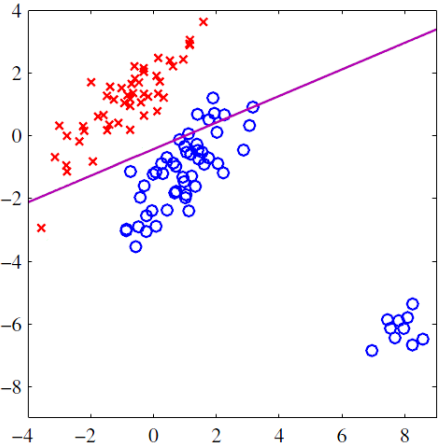
\includegraphics[width=.62\linewidth]{pic/Figure_11.png}
        \end{figure}
        \endminipage
        \vfill
        \begin{tikzpicture}[remember picture,overlay]
            \node[anchor=south west, xshift=0.1cm, yshift=0.22cm] at (current page.south west) {
                \scriptsize Figures adapted from slides of M. Soleymani, Machine Learning course, Sharif University of Technology.
            };
        \end{tikzpicture}
    \end{frame}


    \begin{frame}{An Alternative for SSE Cost Function}
        \begin{itemize}
            \item \textbf{Number of Misclassifications}\itemsep1em
            \medskip
            \begin{itemize}\itemsep0.8em
            \item \textbf{Definition:}
            Measures how many samples are misclassified by the model.

            \item \textbf{Formula:}
            \[
                J(\mathbf{w}) = \sum_{i=1}^{n} \left( \frac{y^{(i)} - \text{sign}(\hat{y}^{(i)})}{2} \right)^2, \quad
                \hat{y}^{(i)} = \mathbf{w}^\top \mathbf{x}^{(i)} + w_0, \quad y^{(i)} \in \{-1, +1\}
            \]

            where the \textbf{sign function} is defined as:
            \[
                \text{sign}(z) =
                \begin{cases}
                    +1 & \text{if } z \ge 0, \\
                    -1 & \text{if } z < 0.
                \end{cases}
            \]

            \item \textbf{Limitations:}
            \begin{itemize}
                \item \justifying \textbf{Piecewise Constant:}
                The cost function is non-differentiable, so optimization techniques (like gradient descent) cannot be directly applied.
            \end{itemize}

            \end{itemize}
        \end{itemize}

        \vfill
        \begin{tikzpicture}[remember picture,overlay]
            \node[anchor=south west, xshift=0.1cm, yshift=0.22cm] at (current page.south west) {
                \scriptsize Figure adapted from Machine Learning and Pattern Recognition, Bishop
            };
        \end{tikzpicture}
    \end{frame}


    \begin{frame}{Perceptron Algorithm}
        \begin{itemize}
            \item \textbf{The Perceptron Algorithm}
            \medskip
            \begin{itemize}\itemsep1em
            \item \justifying \textbf{Purpose}:
            A simple algorithm for binary classification, separating two classes with a linear boundary.
            \end{itemize}
        \end{itemize}
        \begin{figure}
            \centering
            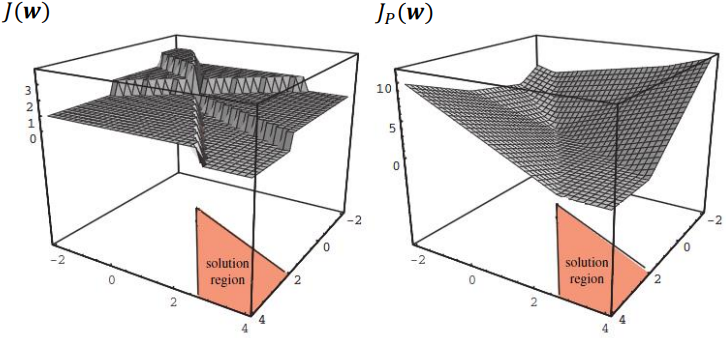
\includegraphics[width=0.7\linewidth]{pic/Figure_13.png}
        \end{figure}
        \vfill
        \begin{tikzpicture}[remember picture,overlay]
            \node[anchor=south west, xshift=0.1cm, yshift=0.22cm] at (current page.south west) {
                \scriptsize Figures adapted from Machine Learning and Pattern Recognition, Bishop
            };
        \end{tikzpicture}
    \end{frame}


    \begin{frame}{Perceptron Criterion}
        \begin{itemize}\itemsep1.2em
        \item \textbf{Cost Function}:
        The perceptron criterion focuses on misclassified points:
        \[
            J_p(\mathbf{w}) = - \sum_{i \in M} y^{(i)} \, \mathbf{w}^T \mathbf{x}^{(i)} \, , \quad y^{(i)} \in \{-1, \, +1\}
        \]
        where \( M \) is the set of misclassified points.
        \item \textbf{Goal}:
        Minimize the loss by correctly classifying all points.
        \end{itemize}
    \end{frame}


    \begin{frame}{Batch Perceptron}
        \begin{itemize}\itemsep1.5em
        \item \justifying \textbf{Batch Perceptron}:
        Updates the weight vector using all misclassified points in each iteration.
        \item \justifying \textbf{Gradient Descent}:
        Adjusting weights in the direction that reduces the loss:
        \[
            \mathbf{w} \leftarrow \mathbf{w} - \eta \nabla_\mathbf{w} \, J_p(\mathbf{w})
        \]
        \[
            \nabla_\mathbf{w} \, J_p(\mathbf{w}) \, = \, - \sum_{i \in M} y_i \mathbf{x}_i
        \]
        \begin{itemize}
            \item Batch Perceptron converges in finite number of steps for linearly separable data.
        \end{itemize}
        \end{itemize}
    \end{frame}

    \begin{frame}{Single-sample Perceptron}
        \begin{itemize}\itemsep1.5em
        \item \justifying \textbf{Single Sample Perceptron}: Updates the weight vector after each individual point.
        \item \textbf{Stochastic Gradient Descent (SGD) Update Rule:}
        \smallskip
        \begin{itemize}\itemsep1em
        \item Using only one misclassified sample at a time:
        \[
            \mathbf{w} \leftarrow \mathbf{w} + \eta y_i \mathbf{x}_i
        \]
        \item Lower computational cost per iteration, faster convergence.
        \item \justifying If training data are linearly separable, the single-sample perceptron is also guaranteed to find a solution in a finite number of steps.
        \end{itemize}
        \end{itemize}
    \end{frame}

    \begin{frame}{Example}
        \begin{itemize}
            \item Perceptron changes \(\mathbf{w}\) in a direction that corrects error.
        \end{itemize}
        \begin{figure}
            \centering
            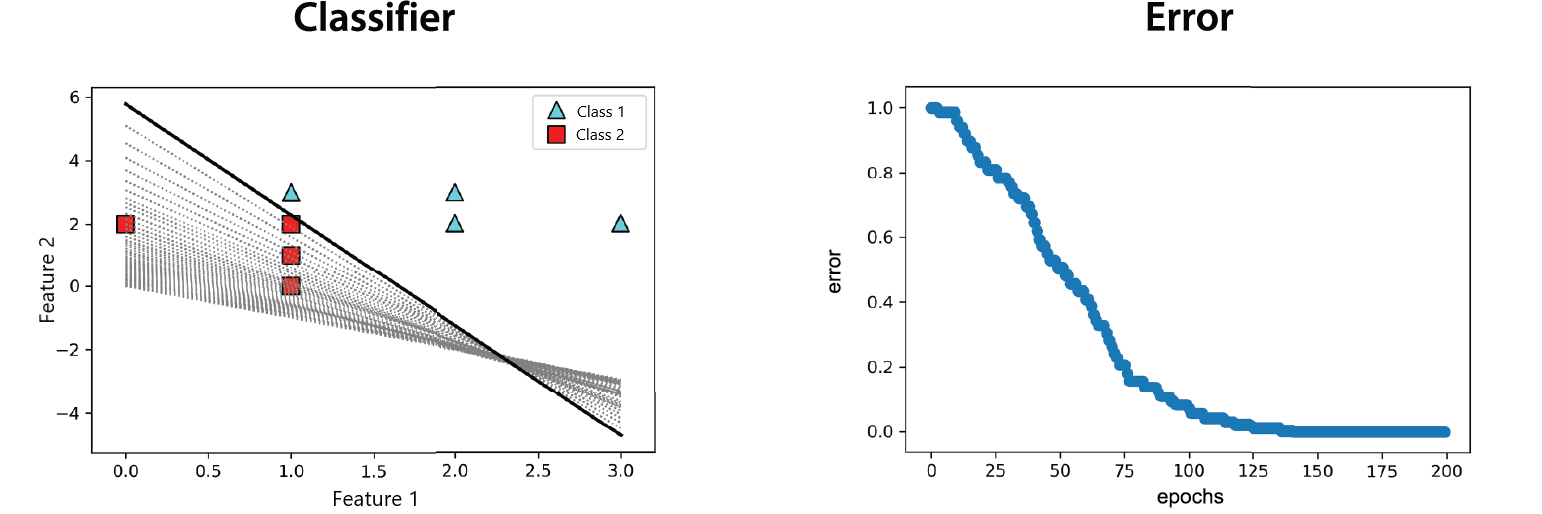
\includegraphics[width=\linewidth]{pic/Figure_14.png}
        \end{figure}
        \vfill
        \begin{tikzpicture}[remember picture,overlay]
            \node[anchor=south west, xshift=0.1cm, yshift=0.22cm] at (current page.south west) {
                \scriptsize Figures adapted from Grokking Machine Learning, L. G. Serrano.
            };
        \end{tikzpicture}
    \end{frame}

    \begin{frame}{Convergence of the Perceptron — Theorem}

        \textbf{Theorem:}
        For linearly separable data with margin $\gamma > 0$ and $\|x_i\| \le R$,
        the Perceptron algorithm makes at most $M \le \tfrac{R^2}{\gamma^2}$ updates.

        \vspace{0.8em}

        \textbf{Notation:}

        \begin{itemize}
            \item Dataset: $D = \{(x_i, y_i)\}_{i=1}^n$, with $x_i \in \mathbb{R}^d$, $y_i \in \{+1, -1\}$.
            \item Weight vector at step $t$: $w_t$, starting from $w_0 = 0$.
            \item Update rule (on misclassified sample):
            $w_{t+1} = w_t + y_t x_t$, where $(x_t, y_t)$ is the misclassified sample at step $t$.
            \item Assume there exists $w^*$ with $\|w^*\| = 1$ that correctly classifies all samples.
            \item Each input is bounded: $\|x_i\| \le R$ (after scaling, $R = 1$).
            \item Margin:
            \[
                \gamma = \min_{(x_i, y_i) \in D} y_i (x_i^\top w^*) > 0.
            \]
        \end{itemize}

    \end{frame}



    \begin{frame}{Convergence of the Perceptron — Proof (1)}

        We analyze the Perceptron as a gradient-descent-like algorithm.
        Each update occurs when a sample is misclassified.

        \begin{enumerate}
            \item Let $(x_t, y_t)$ be the misclassified sample at step $t$.
            The update is
            \[
                w_{t+1} = w_t + y_t x_t.
            \]
            \item By induction, after $M$ updates:
            \[
                w_M = \sum_{t=1}^{M} y_t x_t.
            \]
            \item Inner product with $w^*$:
            \[
                w_M \cdot w^* = \sum_{t=1}^{M} y_t (x_t \cdot w^*) \ge M \gamma.
            \]
        \end{enumerate}

    \end{frame}




    \begin{frame}{Convergence of the Perceptron — Proof (2)}

        \begin{enumerate}
            \setcounter{enumi}{3}
            \item Norm growth:
            \[
                \|w_M\|^2 = \|w_{M-1}\|^2 + 2y_M (w_{M-1}\cdot x_M) + \|x_M\|^2
                \le \|w_{M-1}\|^2 + R^2
            \]
            because $y_M (w_{M-1}\cdot x_M) \le 0$ for a misclassified sample.

            \item By induction:
            \[
                \|w_M\| \le R\sqrt{M}.
            \]

            \item Using Cauchy–Schwarz:
            \[
                M\gamma \le w_M \cdot w^* \le \|w_M\| \|w^*\| \le R\sqrt{M} \implies M \le \frac{R^2}{\gamma^2}.
            \]

        \end{enumerate}

        \vfill
        \footnotesize
        Source: Novikoff (1962), \textit{On Convergence Proofs for Perceptrons};
        M. Collins, \textit{Convergence Proof for the Perceptron Algorithm}, Columbia University.
    \end{frame}




    \begin{frame}{Convergence of Perceptron Cont.}
        \begin{itemize}\itemsep1.5em
        \item \textbf{Non-Linearly Separable Data}:
        When no linear decision boundary can perfectly separate the classes, the Perceptron fails to converge.
        \medskip
        \begin{itemize}\itemsep1em
        \minipage{0.5\textwidth}
        \item If data is not linearly separable, there will always be some points that the model fails to classify.
        \item As a result, the algorithm keeps adjusting the weights to fix the misclassified points, causing it to never converge.
        \item For the data that are not linearly separable due to noise, \textbf{Pocket Algorithm} keeps in its pocket the best \(\mathbf{w}\) encountered up to now.
        \endminipage
        \minipage{0.4\textwidth}
        \hspace{1.5cm}
        \begin{figure}
            \centering
            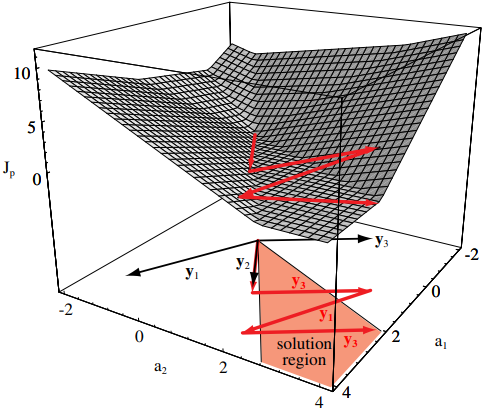
\includegraphics[width=.9\linewidth]{pic/Figure_15.png}
        \end{figure}
        \endminipage
        \end{itemize}
        \end{itemize}
        \vfill
        \begin{tikzpicture}[remember picture,overlay]
            \node[anchor=south west, xshift=0.1cm, yshift=0.22cm] at (current page.south west) {
                \scriptsize Figure adapted from Machine Learning and Pattern Recognition, Bishop
            };
        \end{tikzpicture}
    \end{frame}

    \begin{frame}{Pocket Algorithm}
        \begin{algorithm}[H]
            \caption{Pocket Algorithm}\label{alg:Pocket Algorithm}
            \begin{algorithmic}[1]
                \State \textbf{Initialize} $\mathbf{w}$
                \For{$t = 1$ to $T$}
                    \State \(i \leftarrow t \text{ mod } N\)
                    \If{\(\mathbf{x}^{(i)}\) is misclassified}
                        \State \(\mathbf{w}^{new} \, = \, \mathbf{w} + \eta \mathbf{x}^{(i)}y^{(i)}\)
                        \If{\(E_{train}(\mathbf{w}^{new}) \, < \, E_{train}(\mathbf{w})\)} \Comment{\(E_{train}(\mathbf{w}) \, = \, J_p(\mathbf{w})\)}
                        \State \(\mathbf{w} \, = \, \mathbf{w}^{new}\)
                        \EndIf
                    \EndIf
                \EndFor
            \end{algorithmic}
        \end{algorithm}
    \end{frame}


    \section{Multi-Category Classification}

    \begin{frame}{Multi-Category Classification}
        \begin{itemize}
            \item \textbf{Solutions to multi-category classification problem}:
            \medskip
            \begin{itemize}\itemsep1.5em
            \item Extend the learning algorithm to support multi-class.
            \medskip
            \begin{itemize}\itemsep1em
            \item First, a function \(g_i\) for every class \(C_i\) is found.
            \item Second, \(\mathbf{x}\) is assigned to \(C_i\) if \(g_i(\mathbf{x}) > g_j(\mathbf{x}) \quad \forall i \neq j\)
            \item[] \[\hat{y} \, = \, \argmax_{i=\text{1,...,c}} \, g_i(\mathbf{x})\]
            \end{itemize}
            \item Convert to a set of two-categorical problems.
            \medskip
            \begin{itemize}
                \item Methods like \textbf{One-vs-Rest} or \textbf{One-vs-One}, where each classifier distinguishes between either \textbf{one class and the rest}, or \textbf{between pairs of classes}.
            \end{itemize}
            \end{itemize}
        \end{itemize}
    \end{frame}

    \begin{frame}{Multi-Category Classification: Ambiguity}
        \begin{itemize}
            \item \justifying One-vs-One and One-vs-Rest conversion can lead to regions in which the classification is \textbf{undefined}.
        \end{itemize}
        \vfill
        \minipage{.45\textwidth}
        \begin{figure}[bh]
            \centering
            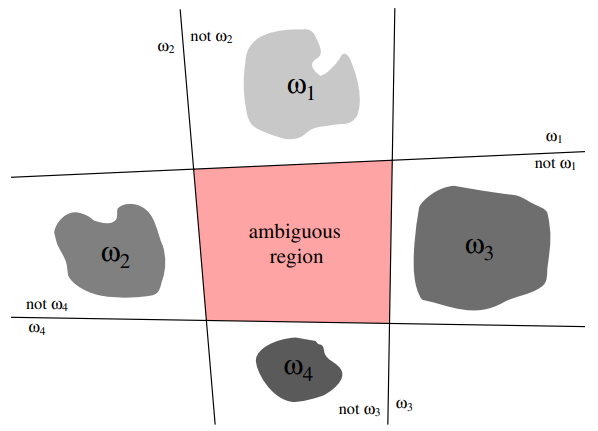
\includegraphics[width=\linewidth]{pic/Figure_6.png}
        \end{figure}
        \endminipage
        \minipage{.45\textwidth}
        \begin{figure}[bh]
            \centering
            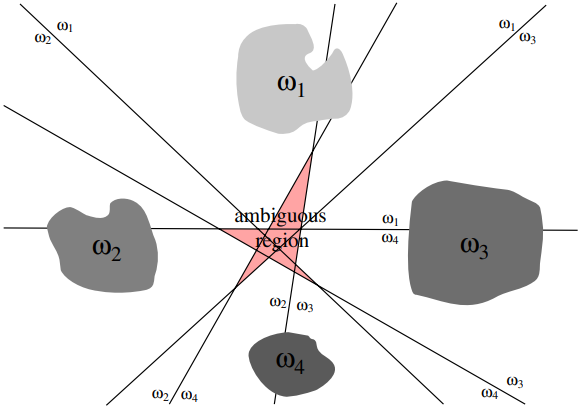
\includegraphics[width=\linewidth]{pic/Figure_7.png}
        \end{figure}
        \endminipage
        \vfill
        \begin{tikzpicture}[remember picture,overlay]
            \node[anchor=south west, xshift=0.1cm, yshift=0.22cm] at (current page.south west) {
                \scriptsize Figures adapted from Machine Learning and Pattern Recognition, Bishop
            };
        \end{tikzpicture}
    \end{frame}


    \begin{frame}{Multi-Category Classification: Linear Machines}
        \begin{itemize}\itemsep1.5em
        \item \justifying \textbf{Linear Machines}: Alternative to One-vs-Rest and One-vs-One methods;
        Each class is represented by its own discriminant function.
        \item \justifying \textbf{Decision Rule:}
        \[\hat{y} \, = \, \argmax_{i=\text{1,...,c}} \, g_i(\mathbf{x})\]
        The predicted class is the one with the highest discriminant function value.
        \item \textbf{Decision Boundary}:
        \(g_i(\mathbf{x}) \, = \, g_j(\mathbf{x})\)
        \[(\mathbf{w}_i - \mathbf{w}_j)^T\mathbf{x} + (w_{0i} - w_{0j}) = 0\]
        \end{itemize}
    \end{frame}


    \begin{frame}{Linear Machines Cont.}
        \begin{center}
            \minipage{.5\textwidth}
            \begin{figure}
                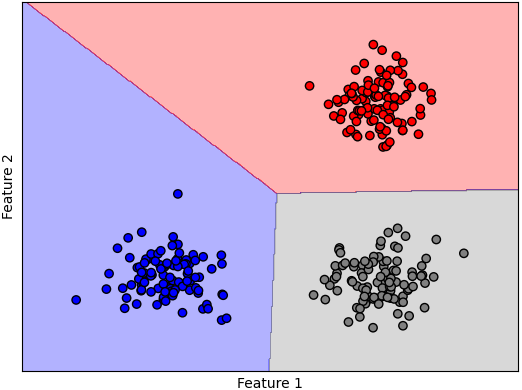
\includegraphics[width=\textwidth]{pic/Figure_9.png}
            \end{figure}
            \endminipage
        \end{center}
        \hspace{4cm}
        \begin{itemize}\itemsep1.5em
        \item \justifying The decision regions of this discriminant are \textbf{convex} and \textbf{singly connected}. Any point on the line between two points within the same region can be expressed as \\
        \(
        \mathbf{x} = \lambda \mathbf{x}_A + (1 - \lambda) \mathbf{x}_B
        \)
        where \( \mathbf{x}_A, \mathbf{x}_B \in C_k \).

        \end{itemize}
    \end{frame}

    \begin{frame}{Multi-Class Perceptron Algorithm}
        \begin{itemize}
            \item \textbf{Weight Vectors}:
            \medskip
            \begin{itemize}\itemsep.8em
            \item Maintain a weight matrix \( W \in \mathbb{R}^{m \times K} \), where \( m \) is the number of features and \( K \) is the number of classes.
            \item Each column \( w_k \) of the matrix corresponds to the weight vector for class \( k \).
            \end{itemize}
        \end{itemize}
        \hspace{4cm}
        \[
            \hat{y} \, = \, \argmax_{i=1,...,c} \, \mathbf{w}_i^T \mathbf{x}
        \]
        \[
            J_p(\mathbf{W}) \, = \, - \sum_{i \in M}(\mathbf{w}_{y^{(i)}} - \mathbf{w}_{\hat{y}^{(i)}})^T\mathbf{x}^{(i)}
        \]
        where \( M \) is the set of misclassified points.
    \end{frame}


    \begin{frame}{Multi-Class Perceptron Algorithm}

        \begin{algorithm}[H]
            \caption{Multi-class perceptron}\label{alg:Multi-class perceptron}
            \begin{algorithmic}[1]
                \State \textbf{Initialize} $\mathbf{W} \, = \, [\mathbf{w}_1 \, , \, ... \, , \, \mathbf{w}_c], \, k \leftarrow 0$
                \While{A pattern is misclassified}
                    \State \(k \leftarrow k \, + \, 1 \text{ mod } N\)
                    \If{\(\mathbf{x}^{(i)}\) is misclassified}
                        \State \(\mathbf{w}_{\hat{y}^{(i)}} \, = \, \mathbf{w}_{\hat{y}^{(i)}} - \eta \mathbf{x}^{(i)}\)
                        \State \(\mathbf{w}_{y^{(i)}} \, = \, \mathbf{w}_{y^{(i)}} + \eta \mathbf{x}^{(i)}\)
                    \EndIf
                \EndWhile
            \end{algorithmic}
        \end{algorithm}

    \end{frame}


    \section{References}


    \begin{frame}{Contributions}
        \begin{itemize}
            \item \textbf{This slide has been prepared thanks to:}
            \medskip
            \begin{itemize}
                \item \href{https://github.com/jefri021}{Erfan Jafari}
                \item {Aida Jalali}
            \end{itemize}
        \end{itemize}

    \end{frame}


    \begin{frame}[allowframebreaks]
        \bibliography{ref}
        \bibliographystyle{ieeetr}
        \nocite{*} % used here because no citation happens in slides
        % if there are too many try use:
        % \tiny\bibliographystyle{alpha}
    \end{frame}

\end{document}